\chapter{VRPTW via AI}
In this chapter, we will review the current end-to-end \gls{ai} methods for solving \gls{vrp} and propose our extension for solving \gls{vrptw}.

Machine learning and artificial intelligence have been replacing many hand-engineered algorithms and providing state-of-the-art results. In recent years, reinforcement learning \ref{rl} and advances in attention models \ref{attention} has shown great promise to disrupt the field of heuristics algorithms \cite{rl-constraint-opt, attention-route, dpdp}. Heuristics algorithms \cite{heuristics-algo} are incomplete methods that can compute solutions efficiently, but are not able to prove the optimality of a solution. Most of the business challenges do not require the most optimal exact solution \cite{excat-algo} but focus on approximation of the optimal solution in a reasonable time.

\section{Related Work}
Researchers have been mainly active in solving general \gls{vrp}...
TODO

\section{Solution}
The end-to-end \gls{ai} method pro solving \gls{vrptw} is extension of the work done by Kool et al. \cite{attention-route}. 

Let us describe the high-level concept behind the method. Consider we have a model as blackbox which takes \gls{vrptw} instance as an input and outputs probabilities for all the \gls{vrptw} nodes. The probability represents which node should be visited next and by following to the most probable node we get a partial solution which will be considered by the blackbox. We iterate this process until all nodes have been visited and we acquire a feasible plan as shown on Figure \ref{fig:attention-route-diagram}.

    \begin{figure}[ht]
        \centering
        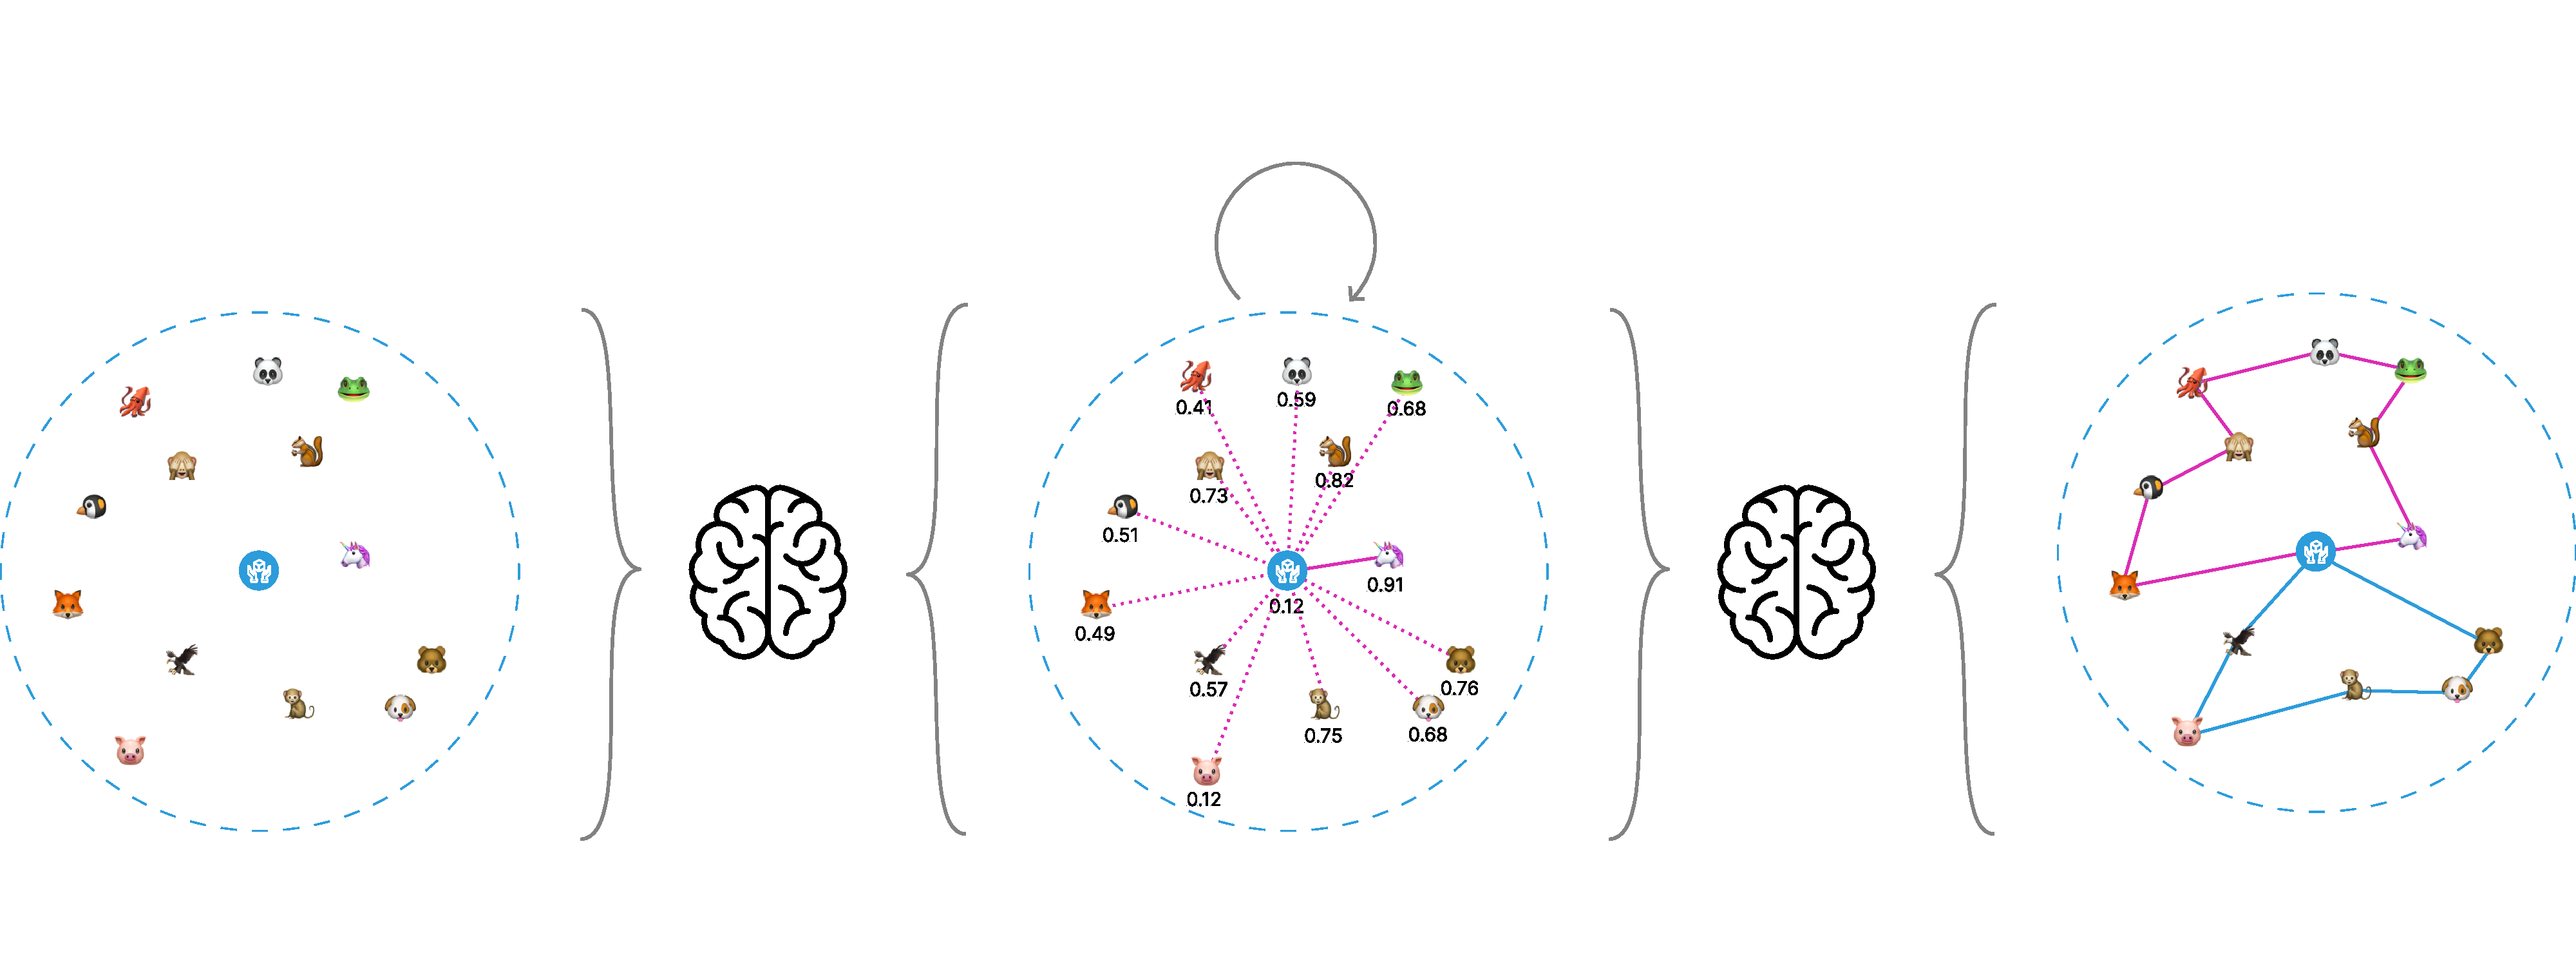
\includegraphics[width=1.0\textwidth]{resources/vrptw-ai/attention-route-diagram.pdf}
        \caption{High-level concept behind the used method.}
        \label{fig:attention-route-diagram}
    \end{figure}

    \subsection{Model Architecture}
    The model architecture by \cite{attention-route} extended by time windows is leveraging recent advancements in attention mechanism. The model is built upon transformers \ref{transformer}, graph attention network \ref{graph-attention-network}, and reinforcement learning \ref{rl}. The network structure is encoder-decoder which is great for solving sequential decision problems. The structural input instance is extracted by the encoder \ref{encoder} and then the solution is incrementally constructed by the decoder \ref{decoder}.
    
    The \gls{vrptw} input instance is consited from
    \begin{itemize}
        \item $X = \{x_1, \cdots, x_n\}$ where $x_i$ is two-dimensional coordinates in the euclidean space.
        \item $x_0$ is the location of depot.
        \item $D = \{d_1, \cdots, d_n\})$ is the demand capacity for each of the locations.
        \item $T = \{(e_1, l_1), \cdots, (e_n, l_n)\})$ is time windows for each of the location where $e_i$ is the beginning and $l_i$ is the end of the considered time window.
    \end{itemize}
    
    The output is the solution of VRPTW instance and is represented as a permutation $\pi$ of locations $X \cup x_0$.
    \begin{itemize}
        \item $\pi = \{\pi_1, \cdots, \pi_T\} \in \{x_0, \cdots, x_n\})$ 
    \end{itemize}
    
    \subsubsection{Encoder}\label{vrptw-encoder}
    The encoder uses graph attention network \ref{graph-attention-network} to embed the node features to graph embedding. Then the decoder architecture is the same as the decoder of transformer \ref{transformer}. Typicaly, the decoder of transformer uses positional encoding \cite{positional-encoding} to embed the input, but in this case it has been replace with \gls{gat} since we deal with graph-based structure.
    
    
    
    \subsubsection{Decoder}\label{vrptw-decoder}
        
    \subsection{Reinforcement Learning}\label{vrptw-rl}
        
    \subsection{Integrating Distance Matrix}
    Multidimensional scaling
